\documentclass{beamer}
    \usetheme{Boadilla}
\usepackage{polyglossia}
    \setmainlanguage{english}
\usepackage{fontspec}
    \setsansfont{Linux Biolinum O}
\usepackage{graphicx}
\usepackage{xcolor}
\usepackage{rotating}
\usepackage{listings}
    \lstset{language=bash,
	basicstyle=\footnotesize\ttfamily\tiny,
	breaklines=true,
	framextopmargin=50pt,
	frame=bottomline,
	backgroundcolor=\color{white!86!black},
	commentstyle=\color{blue},
	keywordstyle=\color{red},
	stringstyle=\color{orange!80!black}}
\usepackage{amsmath}
\usepackage{amssymb}
\usepackage{siunitx}
\usepackage{booktabs}
\usepackage{float}
\usepackage{tabularx}
\usepackage{caption}
\usepackage{subfig}
\usepackage{tikz}
\usepackage{datenumber}
\setbeamertemplate{itemize items}[circle]
\usepackage{hyperref}
     \hypersetup{
     colorlinks=true,
     linkcolor=black,
     filecolor=magenta}

\title{\texorpdfstring{\color{blue!50!black}\textbf{Status report - Thursday}}{}}
\subtitle{ \texorpdfstring{$\chi^{2}$}{Lg}-Distribution and Track Analysis}
\author{Maurice Donner}
\date{July 30, 2020}

\begin{document}

\maketitle

\begin{frame}[fragile]{Tracking}
    Implemented a 3D-Fitting algorithm in python:\\
    \begin{minipage}{.32\textwidth}
	\begin{figure}[H]
	    \centering
	    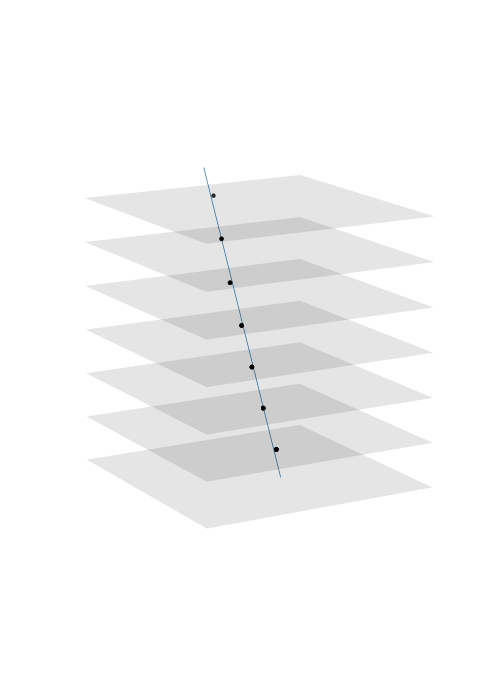
\includegraphics[trim=0 80 0 80,clip,width=\textwidth]{example_1459.png}
	\end{figure}
    \end{minipage}
    \begin{minipage}{.32\textwidth}
	\begin{figure}[H]
	    \centering
	    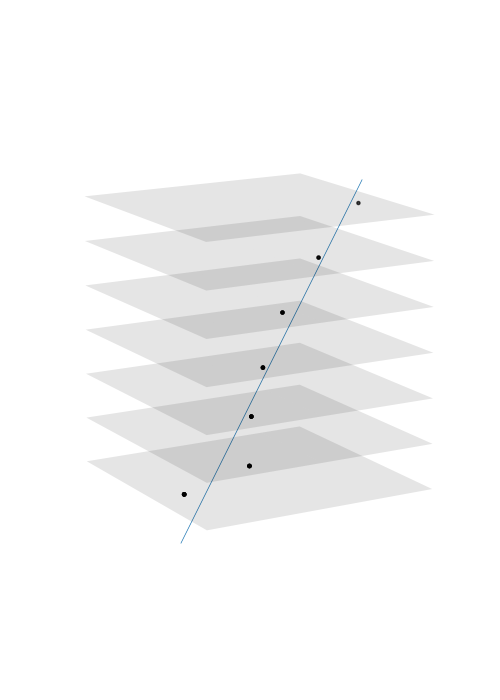
\includegraphics[trim=0 80 0 80,clip,width=\textwidth]{example_112000.png}
	\end{figure}
    \end{minipage}
    \begin{minipage}{.32\textwidth}
	\begin{figure}[H]
	    \centering
	    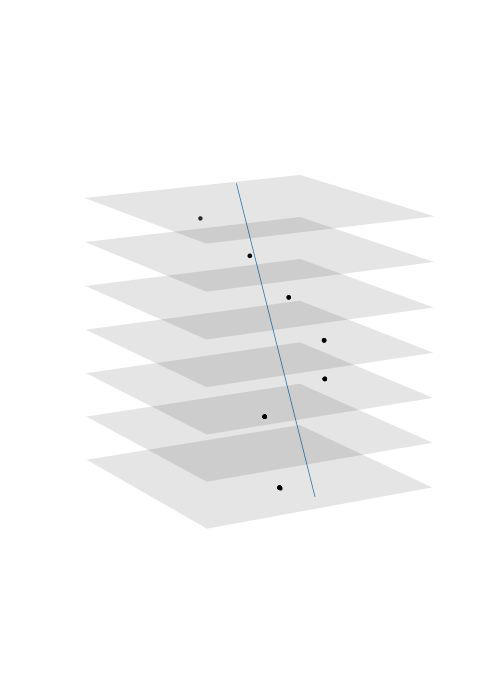
\includegraphics[trim=0 80 0 80,clip,width=\textwidth]{example_290252.png}
	\end{figure}
    \end{minipage}\\
    Using numpy's Singular value decomposition \verb]np.linalg.svd] \\[.1cm]
    \pause
    \( \rightarrow \) Now interested in \( \chi ^2 \) (goodness of fit) \\
    \begin{minipage}{.4\textwidth}
	\begin{figure}[H]
	    \centering
	    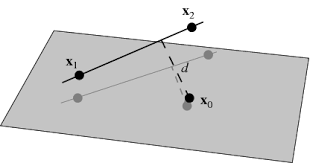
\includegraphics[width=\textwidth]{pointin3d}
	\end{figure}
    \end{minipage}
    \begin{minipage}{.59\textwidth}
	\footnotesize
	\begin{align*}
	    d^2 = \frac{ \left| x_1-x_0 \right|^2 \left| x_2-x_1 \right|^2
		- \left[ \left( x_1-x_0 \right) \cdot \left( x_2-x_1 \right)
		\right]^2}{\left| x_2-x_1 \right|^2}
	\end{align*}
    \end{minipage}

\end{frame}

\begin{frame}{Goodness of Fit}
    \begin{minipage}{.49\textwidth}
    \[ \chi^2 = \sum_{\text{i} = 0} ^6 \frac{ \left(
	    x _{i,\text{hit}} - x _{i,\text{track}} \right) ^2}{
	    \sigma _{i,\text{hit}}} \]
    \end{minipage}
    \begin{minipage}{.49\textwidth}
    i = index of plane
    \end{minipage}\\[.5cm]
    \pause
    \LARGE First look of \( \chi ^{2} \): \\[.5cm]
    \begin{minipage}{.49\textwidth}
    \begin{figure}[H]
	\centering
	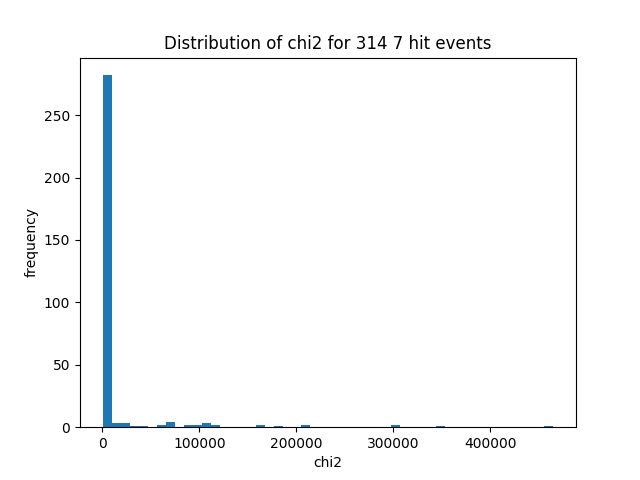
\includegraphics[width=\textwidth]{chi2_firstlook.png}
    \end{figure}
    \end{minipage}
    \begin{minipage}{.49\textwidth}
    \begin{figure}[H]
	\centering
	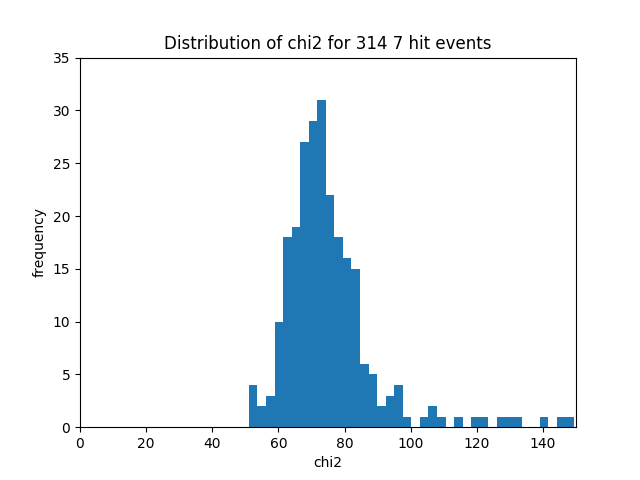
\includegraphics[width=\textwidth]{chi2_secondlook.png}
    \end{figure}
    \end{minipage}
\end{frame}

\begin{frame}{Goodness of Fit}
    \begin{minipage}{.49\textwidth}
    \[ \chi^2 = \sum_{\text{i} = 0} ^6 \frac{ \left(
	    x _{i,\text{hit}} - x _{i,\text{track}} \right) ^2}{
	    \sigma _{i,\text{hit}}} \]
    \end{minipage}
    \begin{minipage}{.49\textwidth}
    i = index of plane
    \end{minipage}\\[.5cm]
    \LARGE First look of \( \chi ^{2} \): \\[.5cm]
    \begin{minipage}{.49\textwidth}
    \begin{figure}[H]
	\centering 
	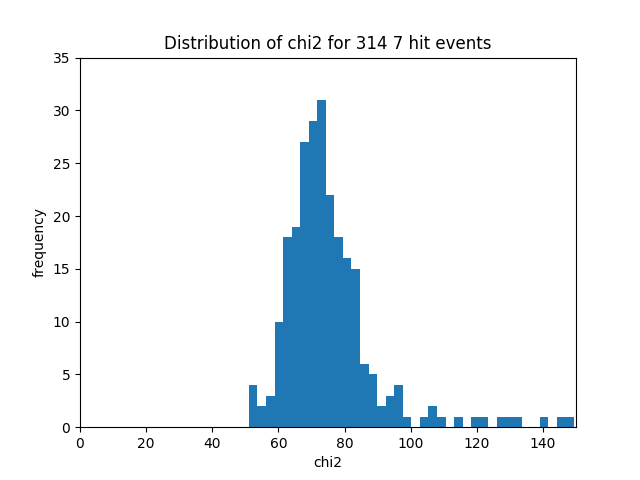
\includegraphics[width=\textwidth]{chi2_secondlook.png}
    \end{figure}
    \end{minipage}
    \begin{minipage}{.45\textwidth}
	\footnotesize
	\begin{itemize}
	    \item Most of the hits are 1 or 2 pixel \( ( \sigma = 0.5 ) \)
	    \item Assume same deviation for all planes \\[.5cm]
	\end{itemize} 
	\tiny
	\( \chi ^2 = 100 \rightarrow \sqrt{100/6 \cdot 0.5} < 3\)
	Pixel \( (90 \si{\micro \meter} )\) 
    \end{minipage}
\end{frame}

\begin{frame}{Goodness of Fit}
    \begin{minipage}{.49\textwidth}
    \[ \chi^2 = \sum_{\text{i} = 0} ^6 \frac{ \left(
	    x _{i,\text{hit}} - x _{i,\text{track}} \right) ^2}{
	    \sigma _{i,\text{hit}}} \]
    \end{minipage}
    \begin{minipage}{.49\textwidth}
    i = index of plane
    \end{minipage}\\[.5cm]
    \LARGE Second look of \( \chi ^{2} \): \\[.5cm]
    \begin{minipage}{.32\textwidth}
    \begin{figure}[H]
	\centering 
	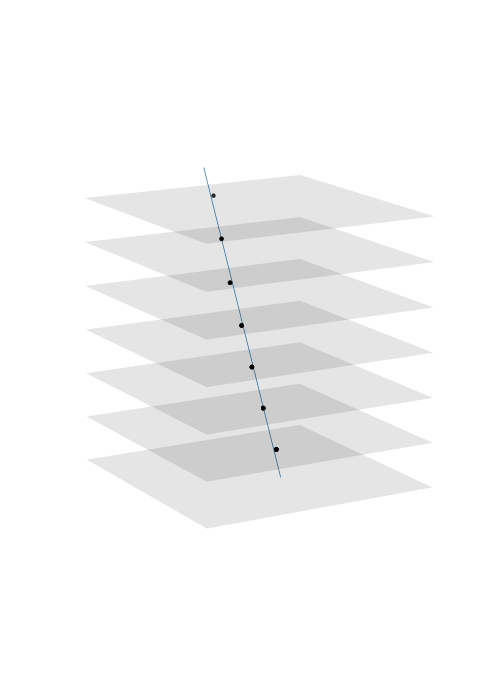
\includegraphics[trim=0 80 0 80,clip,width=\textwidth]{example_1459.png}
	\caption*{\( \chi^2 = 1459 \)}
    \end{figure}
    \end{minipage}
    \begin{minipage}{.32\textwidth}
    \begin{figure}[H]
	\centering
	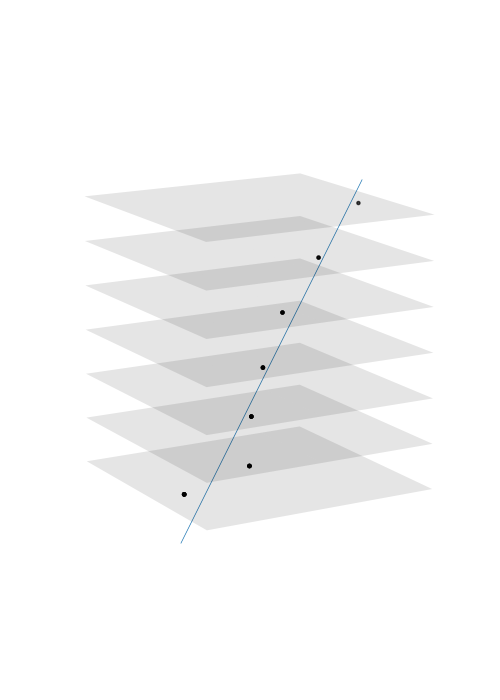
\includegraphics[trim=0 80 0 80,clip,width=\textwidth]{example_112000.png}
	\caption*{\( \chi ^2 = 112000 \)}
    \end{figure}
    \end{minipage}
    \begin{minipage}{.32\textwidth}
    \begin{figure}[H]
	\centering
	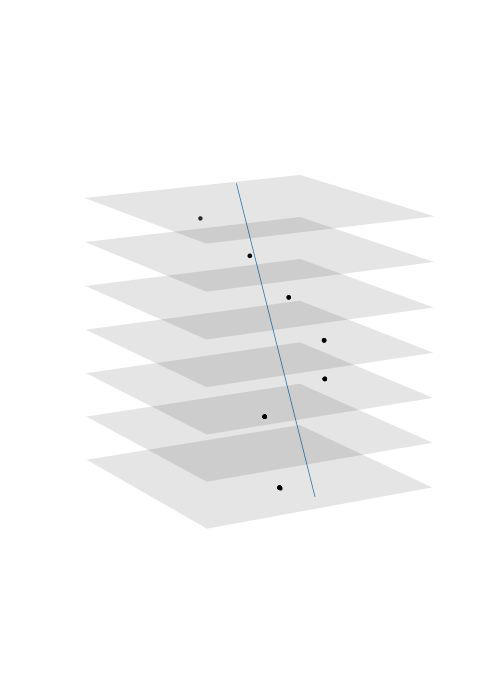
\includegraphics[trim=0 80 0 80,clip,width=\textwidth]{example_290252.png}
	\caption*{\( \chi ^2 = 290252 \)}
    \end{figure}
    \end{minipage}
\end{frame}

\begin{frame}{Taking a closer look at 5+ Events}
    \begin{figure}[H]
	\centering
	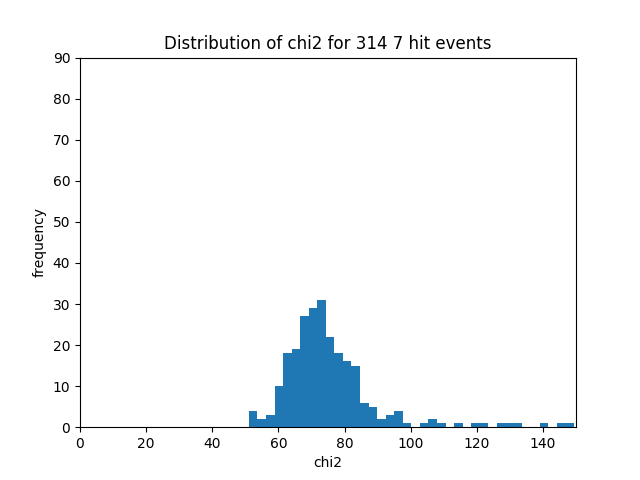
\includegraphics[width=.4\textwidth]{7.png}
    \end{figure}
    \pause
    \begin{tikzpicture}[scale=0.5]
	\draw (0,0);
	\draw[->] (10,1) -- (9,0);
    \end{tikzpicture}\\
    \begin{minipage}{.4\textwidth}
	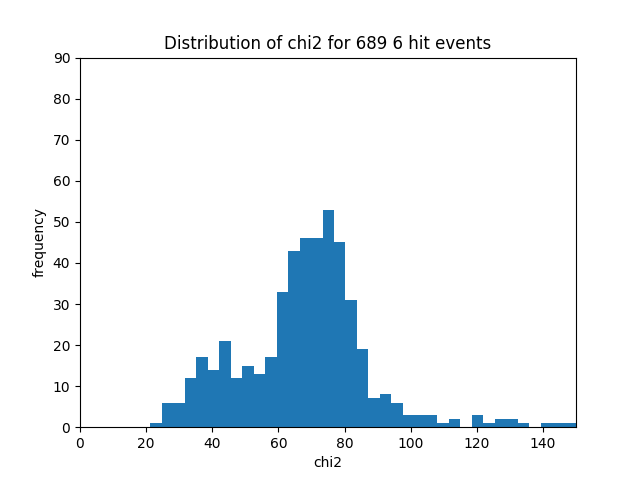
\includegraphics[width=\textwidth]{67.png}
    \end{minipage}
    \pause
    \begin{minipage}{.18\textwidth}
	\centering
	\tikz \draw[->] (0,0) -- (1,0);
    \end{minipage}
    \begin{minipage}{.4\textwidth}
	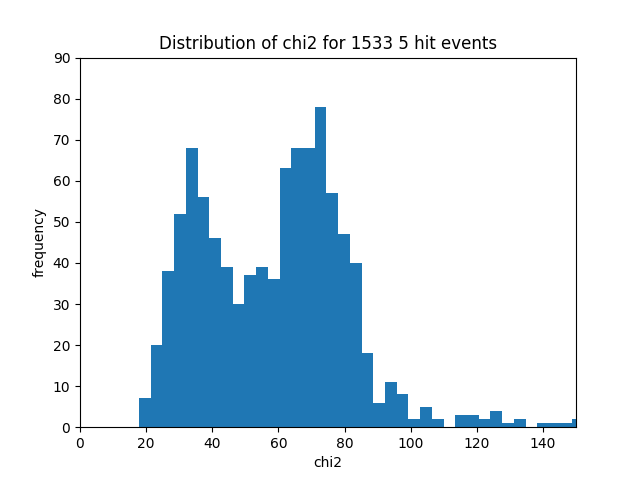
\includegraphics[width=\textwidth]{567.png}
    \end{minipage}
    \pause
    \begin{tikzpicture}[remember picture, overlay]
	\node[xshift=3cm,yshift=-.2cm] at (current page.center)
	{\color{red} Where does this come from?};
	\draw[->,line width=.3mm,color=red] (current page.center) (8.6,3.8) -- (8.6,2.8);
    \end{tikzpicture}
\end{frame}

\begin{frame}{Second peak in \texorpdfstring{\( \chi ^2 \)}{}-Distribution
- What's going on?}
\LARGE Suspicion \\
\normalsize One or more planes is misaligned more than the others, resulting
in a 'higher' Fit-Accuracy for tracks, where that plane is missing \\[.5cm]
- To verify, look at tracks that have a specific \( \chi ^2 \) Value
\pause
\begin{minipage}{.3\textwidth}
    \begin{figure}[H]
	\centering
	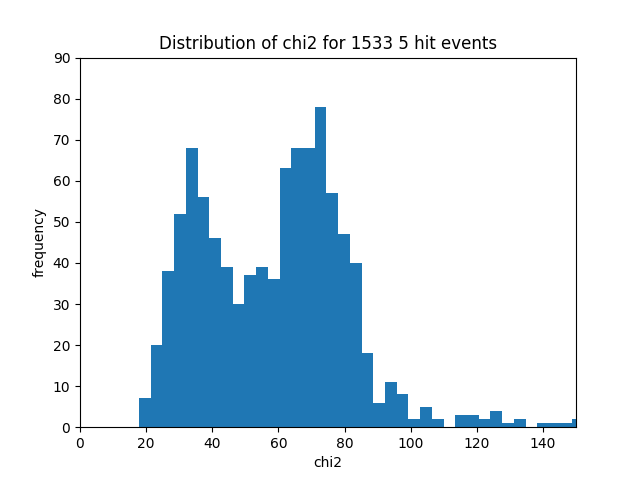
\includegraphics[trim=80 0 160 50,clip,width=\textwidth]{567.png}
    \end{figure}
\end{minipage}
\begin{tikzpicture}[remember picture, overlay]
	\draw[->,line width=.3mm,color=red] (current page.center) (-2.8,2.9) -- (-2.8,2);
\end{tikzpicture}
\begin{minipage}{.49\textwidth}
    \begin{figure}[H]
	\centering
	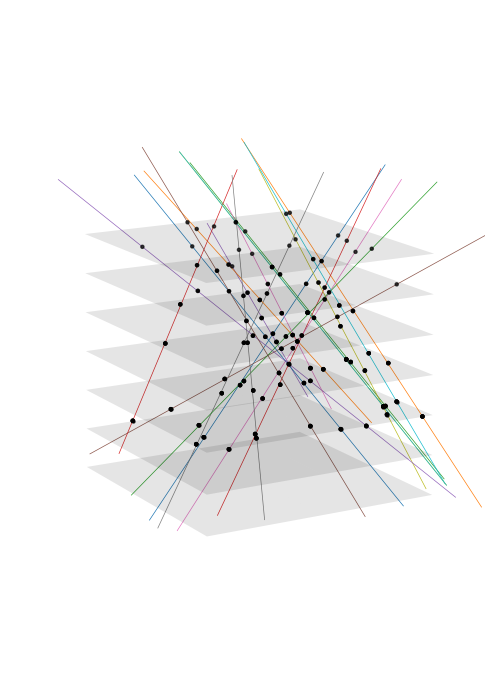
\includegraphics[width=.7\textwidth]{chi2_many_30.png}
    \end{figure}
\end{minipage}
\begin{minipage}{.18\textwidth}
    \footnotesize \begin{turn}{-90}Only little hits on Plane 0 and 1\end{turn}	
\end{minipage}
\end{frame}
\begin{frame}{Second peak in \texorpdfstring{\( \chi ^2 \)}{}-Distribution
- What's going on?}
\LARGE Suspicion \\
\normalsize One or more planes is misaligned more than the others, resulting
in a 'higher' Fit-Accuracy for tracks, where that plane is missing \\[.5cm]
- To verify, look at tracks that have a specific \( \chi ^2 \) Value
\begin{minipage}{.3\textwidth}
    \begin{figure}[H]
	\centering
	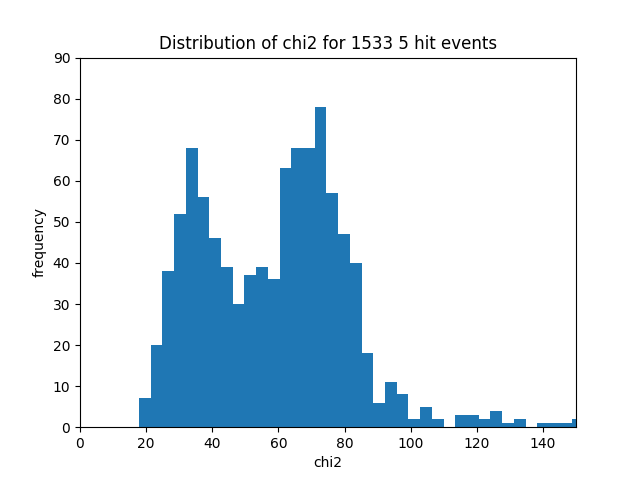
\includegraphics[trim=80 0 160 50,clip,width=\textwidth]{567.png}
    \end{figure}
\end{minipage}
\begin{tikzpicture}[remember picture, overlay]
	\draw[->,line width=.3mm,color=red] (current page.center) (-1.4,2.9) -- (-1.4,2.2);
\end{tikzpicture}
\begin{minipage}{.49\textwidth}
    \begin{figure}[H]
	\centering
	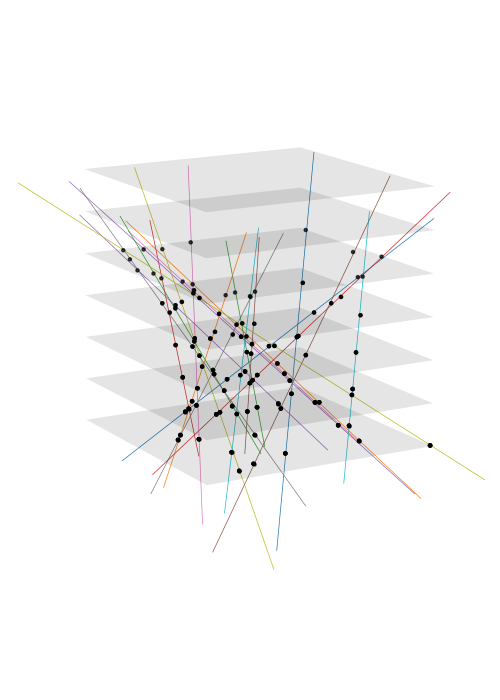
\includegraphics[width=.7\textwidth]{chi2_many_75.png}
    \end{figure}
\end{minipage}
\begin{minipage}{.18\textwidth}
    \footnotesize \begin{turn}{-90}Only little hits on Plane 5 and 6\end{turn}	
\end{minipage}
\pause
\begin{tikzpicture}[remember picture, overlay]
	\node[xshift=0,yshift=-25,rotate=-10,scale=3,color=red] at (current page.center)
	{Need better alignment...};
\end{tikzpicture}
\end{frame}

\end{document}
